\chapter{Logiciel}
Le logiciel développé dans le cadre de ce travail a pour objectifs de collecter, traiter, afficher, et sauvegarder les données mesurées par le capteur.
Le logiciel fourni par le fabriquant permet déjà d'utiliser le capteur, cependant il manque certaines fonctionnalités. Le nouveau logiciel apporte donc des fonctionnalités importantes du logiciel, on peut citer l’ouverture dans une seule fenêtre unique, ce qui facilite la navigation et la lisibilité.
L'utilisateur a un contrôle total sur les mesures : il peut notamment ajuster la précision ainsi que la largeur de bande de la mesure (en Hz).
Il peut aussi choisir non seulement quel harmonique on désire mesurer mais il est possible de choisir plusieurs harmoniques en même temps.

\section{Choix du langage de programmation}

Les critères de sélection du langage de programmation pour le développement du logiciel sont les suivants :

\begin{table}[H]
    \centering
    \begin{tabular}{|p{6cm}|c|c|c|c|}
        \hline
        \textbf{Critère} & \textbf{C} & \textbf{C++} & \textbf{C\#} & \textbf{Python} \\
        \hline
        Compatible avec les fonctions du fabricant QCM & Non & Non & Non & Oui \\
        \hline
        Traitement et affichage des données en temps réel & Oui & Oui & Oui & Oui \\
        \hline
        Facile à apprendre et à utiliser & Non & Non & Moyen & Oui \\
        \hline
        Gestion de la communication série avec le capteur & Oui & Oui & Oui & Oui \\
        \hline
        Multi-plateforme & Oui & Oui & Moyen & Oui \\
        \hline
    \end{tabular}
    \caption{Comparatif des langages selon les critères de sélection}
    \label{tab:comparatif_langages}
\end{table}

Le langage de programmation choisi pour le développement du logiciel est Python.  
Ce choix s’explique par le fait qu’il est le seul à répondre à l’ensemble des critères de sélection. C’est également le langage utilisé par le fabricant pour le développement de son logiciel, ce qui facilite grandement l’adaptation et la réutilisation des fonctions déjà existantes.  
Par ailleurs, Python est un langage largement enseigné dans les milieux scientifiques et techniques, ce qui facilite sa prise en main par de futurs développeurs.


\section{Architecture du logiciel}
\subsection{Paradigmes de programmation}

\begin{table}[H]
    \centering
    \begin{tabular}{|l|c|c|c|}
        \hline
        \textbf{Critère} & \textbf{Procédural} & \textbf{Fonctionnel} & \textbf{Orienté objet} \\
        \hline
        Facilité de prise en main & 3 & 1 & 2 \\
        Organisation du code / lisibilité & 1 & 2 & 3 \\
        Adaptation à une interface graphique & 2 & 1 & 3 \\
        Évolutivité / maintenance & 1 & 2 & 3 \\
        Réutilisabilité du code & 1 & 2 & 3 \\
        Parallélisation des tâches & 1 & 3 & 2 \\
        Rapidité d'exécution & 3 & 2 & 1 \\
        \hline
        \textbf{Note totale} & \textbf{12} & \textbf{14} & \textbf{17} \\
        \hline
    \end{tabular}
    \caption{Évaluation des paradigmes pour un logiciel de mesure avec interface graphique (classement de 1 à 3)}
    \label{tab:comparatif_paradigmes}
\end{table}

Le tableau \ref{tab:comparatif_paradigmes} présente une évaluation des paradigmes de programmation pour un logiciel de mesure avec interface graphique.

Le paradigme orienté objet obtient la meilleure note totale, ce qui en fait le choix privilégié pour ce logiciel. Il se distingue notamment par sa capacité à organiser le code de manière claire, à modéliser des composants complexes (comme des capteurs ou des interfaces utilisateurs) et à faciliter l’évolution du logiciel grâce à l’encapsulation, l’héritage et la réutilisabilité.

Ces caractéristiques sont particulièrement adaptées dans le cadre d'une application de mesures où l’on doit, à la fois gérer l’état interne de l’instrument, l’interface graphique, la communication avec le capteur et structurer le code.

Bien que le paradigme fonctionnel soit intéressant pour la parallélisation ou le traitement des données, et que le paradigme procédural soit plus simple à mettre en place pour des scripts très courts, ils restent moins adaptés à la complexité et à la maintenabilité attendues dans ce projet.

\subsection{Diagramme de classes}

La figure \ref{uml.drawio} présente le diagramme de classes du logiciel développé. Ce diagramme illustre la structure orientée objet retenue ainsi que la répartition des fonctionnalités entre les différentes classes.

Chaque objet est conçu pour assumer une responsabilité bien précise, ce qui permet de structurer le code de manière claire, modulaire et évolutive. Les classes principales sont les suivantes :

\begin{itemize}[label=\textbullet]
  \item \textbf{SerialConnection}~: abstraite, contient les méthodes standard de communication série.
  \item \textbf{QCMSerial}~: hérite de \textbf{SerialConnection} et est responsable de l’établissement de la connexion ainsi que de la lecture des données spécifiques à une microbalance.
  \item \textbf{PT100Signal}~: hérite de \textbf{SerialConnection} et est responsable de l’établissement de la connexion ainsi que de la lecture des données spécifiques à une sonde de température PT100.
  \item \textbf{Signal}~: se charge du traitement du signal (filtrage, extraction de caractéristiques, etc.).
  \item \textbf{Parameter}~: regroupe l’ensemble des paramètres associés à un signal, comme la fréquence d’amplitude maximale, l'amplitude maximale, ou encore la température du QCM.
  \item \textbf{Parameters}~: regroupe une liste d’objets \textbf{Parameter} ; elle permet de sauvegarder, charger et extraire les paramètres de mesure.
  \item \textbf{Settings}~: gère les paramètres de configuration de la prise de mesures.
  \item \textbf{Mesure}~: joue un rôle central en coordonnant les autres objets. Elle représente l’ensemble du processus de mesure, de l’acquisition à l’analyse. Elle contient tous les signaux mesurés ainsi que les paramètres de mesure.
\end{itemize}

\fig[H, width=\textwidth]{Diagramme UML de classes}{uml.drawio}

\newpage

\section{Mesures}

Les mesures se déroulent en deux étapes.

Dans un premier temps, le capteur effectue une mesure de calibration. Cette mesure consiste à balayer toute la plage de fréquences allant de 1 à 5{,}5~MHz avec un pas entre les points de mesure de 1~kHz (voir figure~\ref{fig:calibration 5MHz plot}).  
L’objectif de cette étape est d’identifier automatiquement les fréquences de résonance du quartz. Pour ce faire, il est essentiel de détecter la fréquence fondamentale du quartz afin de déterminer s’il s’agit d’un quartz de 10~MHz ou de 5~MHz.  
La méthode consiste à repérer la position du premier pic de résonance. Une fois cette fréquence déterminée, le programme peut ensuite rechercher toutes les fréquences de résonance : on en attend trois pour un quartz à 10~MHz et six pour un quartz à 5~MHz.

\begin{figure}[H]
    \centering
    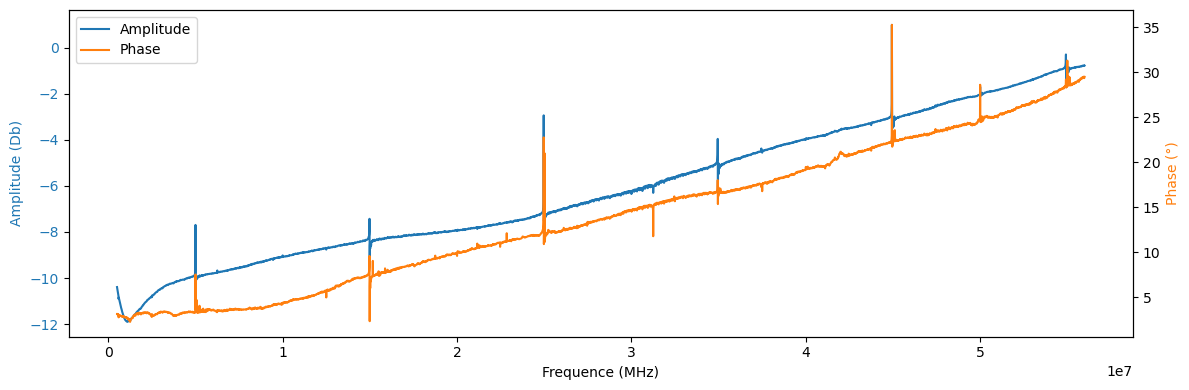
\includegraphics[width=\textwidth]{assets/figures/5MhzCalibration.png}
    \caption{Signal de calibration du capteur QCM 5MHz comportant 6 pics de résonance}
    \label{fig:calibration 5MHz plot}
\end{figure}

\begin{figure}[H]
    \centering
    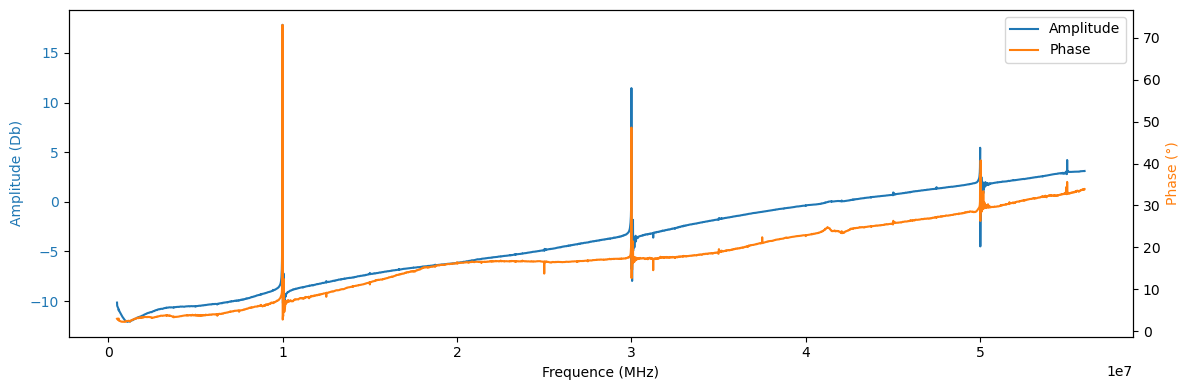
\includegraphics[width=\textwidth]{assets/figures/10MHzCalibration.png}
    \caption{ignal de calibration du capteur QCM 10MHz comportant 3 pics de résonance}
    \label{fig:harmonic 10MHz Calibration}
\end{figure}

La deuxième étape consiste à mesurer plus précisément les pics de résonance (figure~\ref{fig:harmonic 5MHz plot}) identifiés lors de la mesure de calibration.  
Pour cela, une fenêtre est choisie autour de chaque pic de résonance.  
Dans le cas de la figure~\ref{fig:harmonic 5MHz plot}, la fenêtre s’étend de \(-5000\)~Hz à \(+15000\)~Hz autour de la fréquence de calibration. Le pas de mesure est de 20~Hz, afin d’obtenir une précision maximale.

\begin{figure}[H]
    \centering
    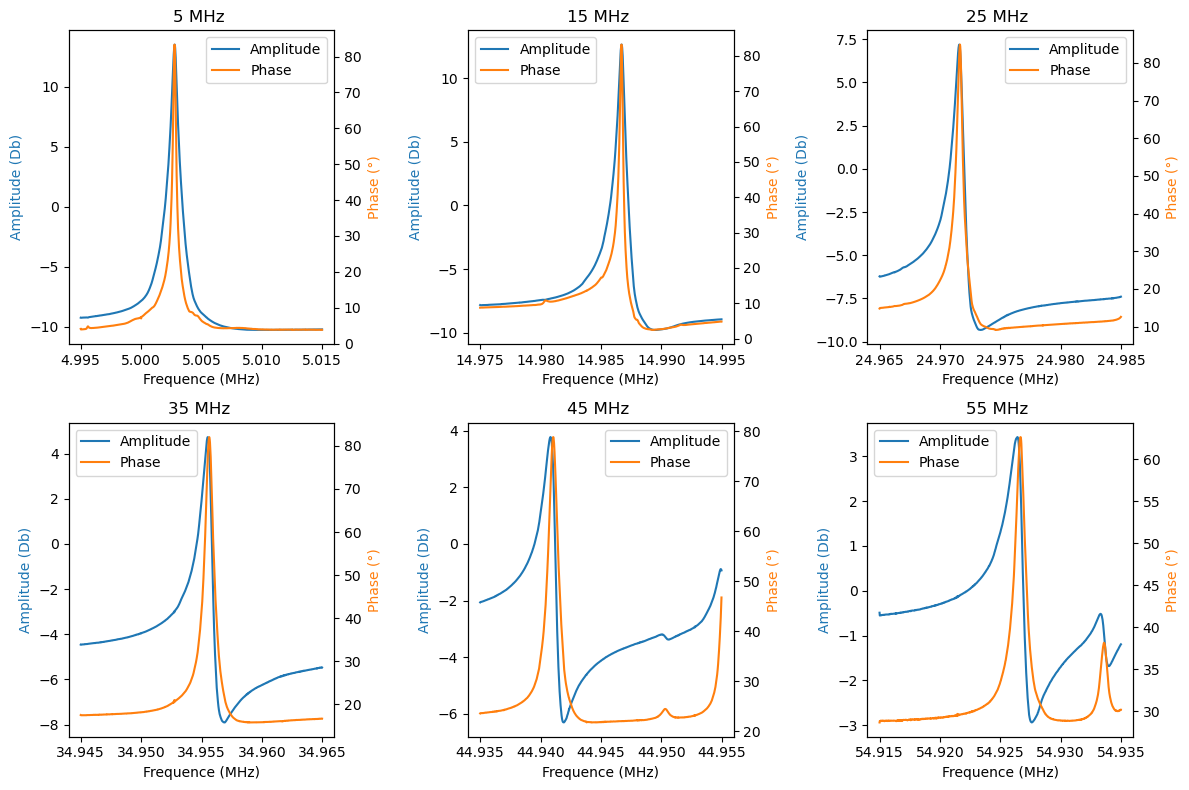
\includegraphics[width=\textwidth]{assets/figures/5MhzPeak.png}
    \caption{Zoom sur les pics de résonance du quartz 5~MHz.}
    \label{fig:harmonic 5MHz plot}
\end{figure}

\begin{figure}[H]
    \centering
    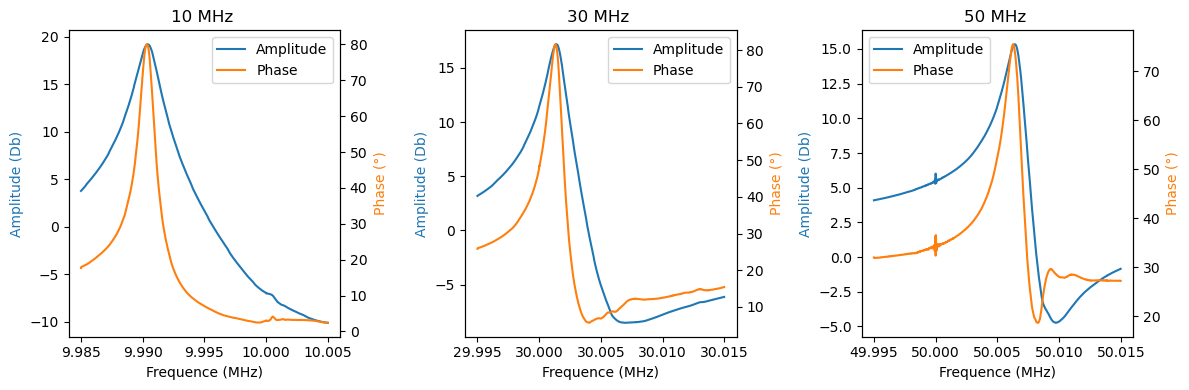
\includegraphics[width=\textwidth]{assets/figures/10MhzPeak.png}
    \caption{Zoom sur les 3 premières harmoniques du quartz 10~MHz.}
    \label{fig:harmonic 10MHz plot}
\end{figure}

\section{Sélection des mesures}

Depuis le menu, il est possible d'accéder à la fenêtre de sélection des paramètres de mesure (voir figure~\ref{fig:paramerter window}).  
Les paramètres suivants peuvent être modifiés par l'utilisateur selon ses besoins :

\begin{itemize}[label=\textbullet]
    \item \textbf{Limite du nombre de mesures} : nombre maximum de mesures à effectuer. Si la limite est désactivée, l'utilisateur devra appuyer sur "Stop" pour arrêter la mesure.
    
    \item \textbf{Pas de la mesure de calibration} : pas de mesure (en Hz) utilisé lors de la calibration.
    
    \item \textbf{Décalage négatif des mesures de pic} : décalage en Hz appliqué avant la fréquence de résonance détectée.
    
    \item \textbf{Décalage positif des mesures de pic} : décalage en Hz appliqué après la fréquence de résonance détectée.
    
    \item \textbf{Pas des mesures de pic} : pas de mesure (en Hz) utilisé pour le balayage autour des pics de résonance.
    
    \item \textbf{Harmonique(s)} : harmonique(s) à mesurer. Il est possible d'en sélectionner plusieurs simultanément.
    
    \item \textbf{Temps d'attente} : temps en secondes entre chaque mesure.
    
    \item \textbf{Calibration par la phase} : si cette option est activée, la calibration se fait en fonction de la phase du signal ; sinon, elle se fait en fonction de l'amplitude.
\end{itemize}

\begin{figure}[H]
    \centering
    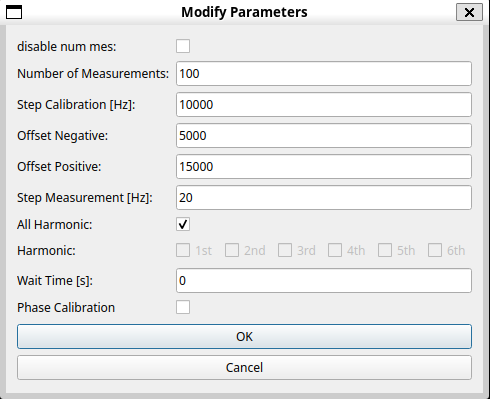
\includegraphics[width=0.6\textwidth]{assets/figures/Parameter_window.png}
    \caption{Fenêtre de sélection des paramètres de mesure}
    \label{fig:paramerter window}
\end{figure}

\section{Affichage des données} 

Le logiciel dispose de deux fenêtres pour afficher les données.

La première est la fenêtre de mesures (figure~\ref{fig:main window}), qui est la fenêtre principale du logiciel depuis laquelle il est possible d'observer l'évolution des données.  
Cette fenêtre est composée de plusieurs parties :

\begin{enumerate}
    \item Une barre d'outils permettant de se connecter au capteur, de lancer et d'arrêter les mesures.
    \item L'affichage des signaux d'amplitude et de phase du signal de calibration.
    \item L'affichage des signaux d'amplitude et de phase des harmoniques mesurées. Ce groupe est dynamique selon le nombre d'harmoniques choisies.
    \item L'affichage de la fréquence de la première harmonique mesurée en fonction du temps, ainsi que la température du capteur intégré.
    \item La liste des mesures effectuées, qui permet d'afficher les harmoniques de chaque mesure lorsque l'utilisateur clique dessus.
    \item Différents messages pour informer l'utilisateur de l'état du logiciel, de l'état des connexions entre l'ordinateur et les capteurs, ainsi que de l'état des mesures.
\end{enumerate}

\begin{figure}[H]
    \centering
    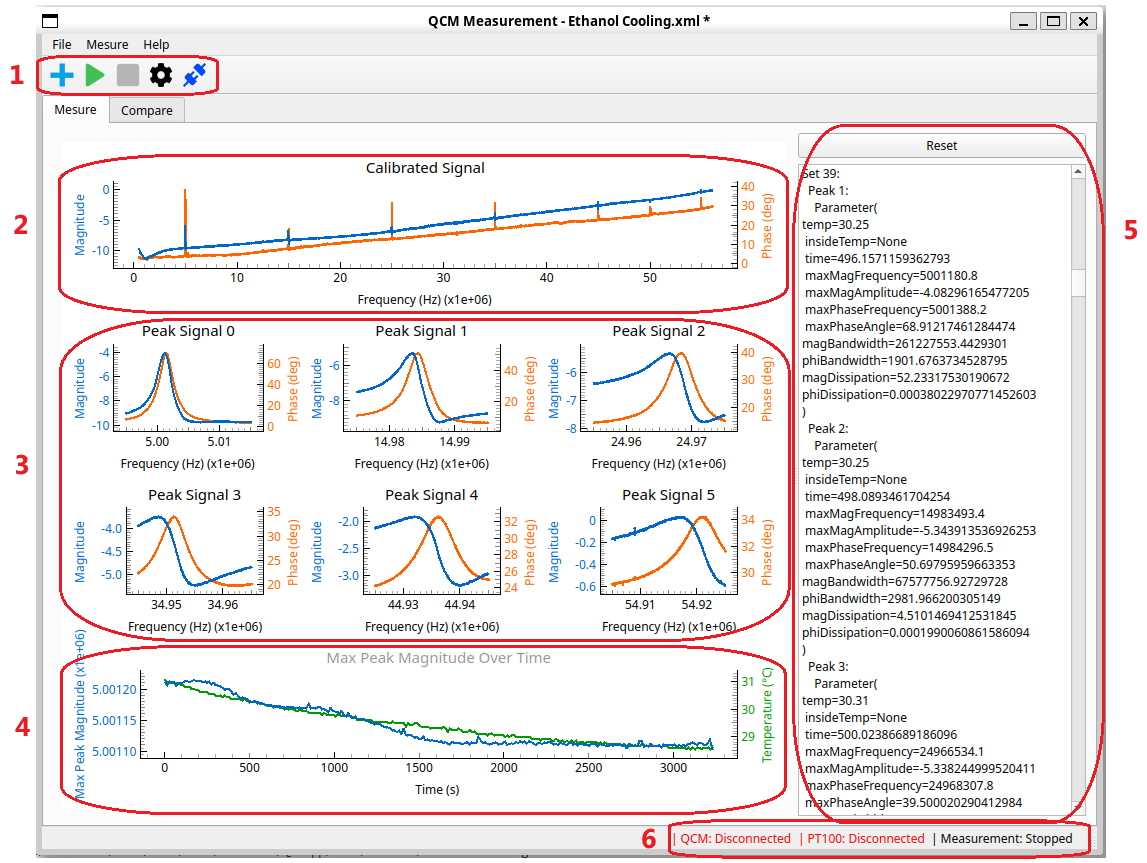
\includegraphics[width=\textwidth]{assets/figures/Programme_.png}
    \caption{Fenêtre principale du logiciel de mesure}
    \label{fig:main window}
\end{figure}

La deuxième fenêtre est la fenêtre de visualisation des données (figure~\ref{fig:plot window}).  
Elle permet de visualiser les données mesurées sous forme de graphiques.  
Il est possible de choisir n'importe quel paramètre de la mesure à afficher sur l'axe des abscisses et n'importe quel paramètre à afficher sur l'axe des ordonnées.  
Il est également possible de choisir l'harmonique à afficher.

\begin{enumerate}
    \item Une barre d'outils est également disponible dans cet onglet.
    \item Une série de menus et de boutons permet de choisir les paramètres à afficher sur les axes.
    \item Un grand graphique au centre de la fenêtre permet de visualiser les données mesurées.
    \item La barre de statut en bas de la fenêtre affiche les mêmes informations que l'onglet de mesures.
\end{enumerate}

\begin{figure}[H]
    \centering
    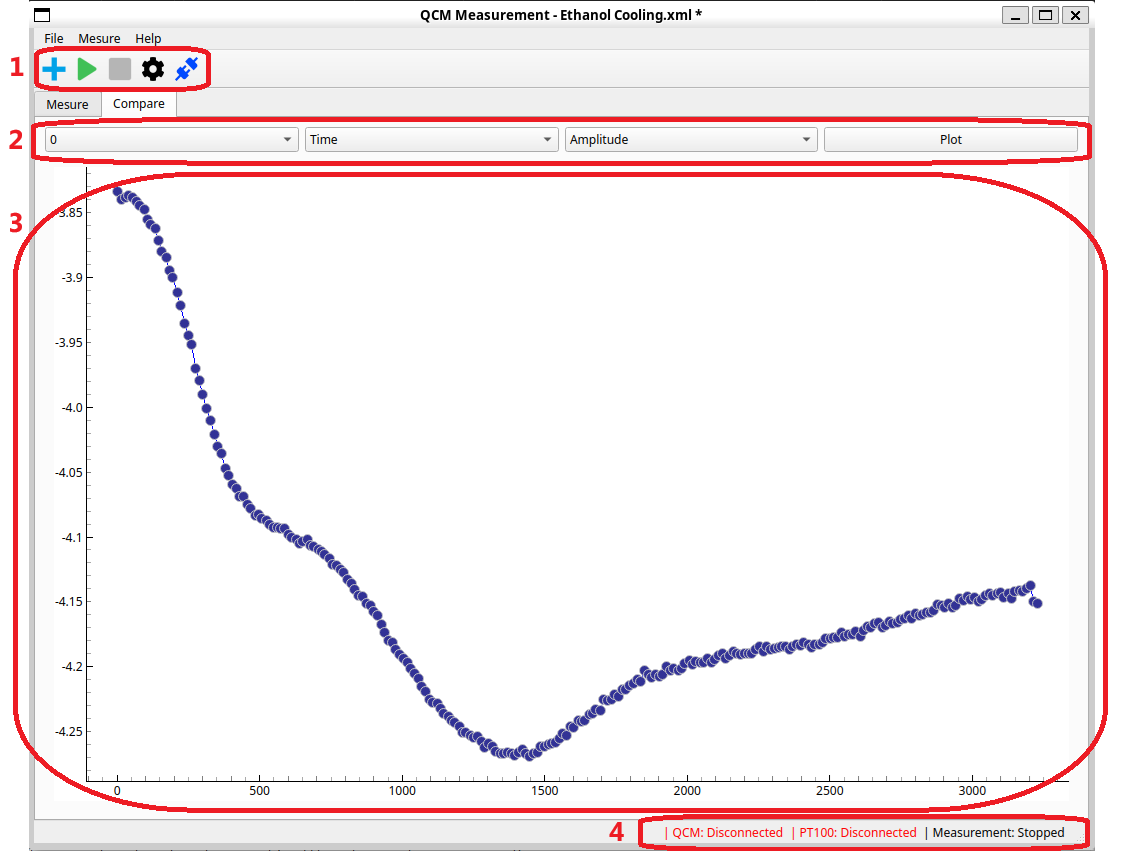
\includegraphics[width=\textwidth]{assets/figures/Plot_window_.png}
    \caption{Fenêtre de visualisation des données}
    \label{fig:plot window}
\end{figure}

\section{Communication avec le capteur}

Pour communiquer avec le capteur, une connexion série est établie. Cette connexion permet d'envoyer des commandes et de recevoir des données.

L’envoi des commandes se fait au moyen d’une chaîne de caractères. La commande comprend la fréquence de début, la fréquence de fin et le pas de la mesure. Les données sont séparées par un point-virgule (\texttt{;}). La trame est terminée par un retour à la ligne (\texttt{\textbackslash n}).

\begin{minted}{bash}
500000;55990000;10000

9985000;10004980;20

29995000;30014980;20
\end{minted}

Le capteur répond avec les données mesurées. Ces données sont formatées avec l'amplitude en premier, suivie par la phase, séparées par un point-virgule (\texttt{;}). Les points de mesure sont séparés par un retour à la ligne (\texttt{\textbackslash n}).

Pour annoncer que la mesure est terminée, le capteur envoie la température en degrés Celsius, suivie d’un point-virgule (\texttt{;}) et de la lettre \texttt{s}.

\begin{minted}{bash}
2968.94;3450.61\n

25.81;s
\end{minted}

La conversion des valeurs brutes issues de l'ADC en unités d'amplitude se fait selon l'équation~\ref{eq:adc_conversion_Amplitude}, et la conversion de la phase selon l'équation~\ref{eq:adc_conversion_phase}.

\begin{equation}
A_i = \frac{\left( \left( x_i \times \frac{k}{2} \right) - V_{\text{CP}} \right)}{0.03}
\label{eq:adc_conversion_Amplitude}
\end{equation}

\begin{equation}
\phi_i = \frac{\left( \left( x_i \times \frac{k}{1.5} \right) - V_{\text{CP}} \right)}{0.01}
\label{eq:adc_conversion_phase}
\end{equation}

\begin{equation}
k = \frac{V_{\text{max}}}{N_{\text{max}}}
\label{eq:adc_conversion}
\end{equation}

où :
\begin{itemize}[label=\textbullet]
    \item $x_i$ : valeur brute de l'ADC pour l'échantillon $i$,
    \item $V_{\text{max}}$ : tension maximale mesurable par l'ADC (ici $3.3\,\mathrm{V}$),
    \item $N_{\text{max}}$ : valeur maximale du codeur ADC (ici $8192$, correspondant à un ADC sur 13 bits),
    \item $V_{\text{CP}}$ : tension de référence (0,9\,V),
    \item $y_i$ : valeur convertie (en unité physique finale).
    \item $k$ : coefficient de conversion de l'ADC, qui dépend de la tension maximale mesurable et de la résolution de l'ADC.   
\end{itemize}

\section{Connexion}

\begin{figure}[H]
    \begin{minipage}{0.64\textwidth}
        La fenêtre de connexion, figure~\ref{fig:connection window}, permet de connecter le capteur QCM et la sonde de température PT100.
        Depuis cette interface, l'utilisateur peut choisir le port série auquel le capteur est connecté, ainsi que le port série de la sonde de température.
        Pour que la sonde de température soit activée, il est nécessaire d'activer le capteur de température dans les paramètres de mesure.
    \end{minipage}\hfill
    \begin{minipage}{0.30\textwidth}
        \centering
        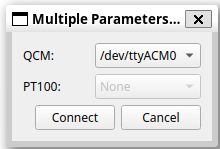
\includegraphics[width=\textwidth]{assets/figures/ConnectionDialogue.png}
        \caption{Fenêtre de connexion}
        \label{fig:connection window}
    \end{minipage}
\end{figure}

\begin{figure}[H]
    \begin{minipage}{0.64\textwidth}
        La fenêtre d'attente de connexion, figure~\ref{fig:connecting window}, a pour objectif de signaler à l'utilisateur que le logiciel est en train d'établir la connexion avec le capteur QCM et la sonde de température PT100.
        Pour ce faire, un bandeau de progression est affiché, ainsi qu'un message d'information.

        Il est important de noter que, pour assurer la fluidité de l'interface graphique, le logiciel utilise un thread séparé pour établir la connexion.
    \end{minipage}\hfill
    \begin{minipage}{0.30\textwidth}
        \centering
        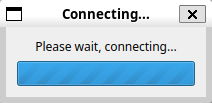
\includegraphics[width=\textwidth]{assets/figures/Connecting.png}
        \caption{Fenêtre d'attente de connexion}
        \label{fig:connecting window}
    \end{minipage}
\end{figure}

La connexion se déroule en deux étapes.
Dans un premier temps, le logiciel tente de se connecter au capteur QCM. Si la connexion échoue, un message d'erreur est affiché, figure~\ref{fig:connection fail}.
Dans un second temps, le logiciel vérifie que la connexion a été établie avec le bon matériel.

Pour le QCM, le logiciel envoie une requête de mesure puis attend deux chiffres séparés par un point-virgule (\texttt{;}) et terminés par un retour à la ligne (\texttt{\textbackslash n}).
Pour la sonde de température, le logiciel envoie une requête de mesure puis attend un chiffre suivi d'un retour à la ligne (\texttt{\textbackslash n}).

\begin{figure}[H]
    \begin{minipage}{0.64\textwidth}
        En cas d’échec de la connexion, la fenêtre de connexion, figure~\ref{fig:connection fail}, affiche un message d'erreur indiquant que la connexion a échoué.
        Une fois le message d'erreur validé par l'utilisateur, le logiciel revient à la fenêtre de connexion, figure~\ref{fig:connection window}.
    \end{minipage}\hfill
    \begin{minipage}{0.30\textwidth}
        \centering
        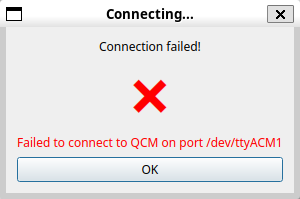
\includegraphics[width=\textwidth]{assets/figures/ConnectionFail.png}
        \caption{Fenêtre de connexion échouée}
        \label{fig:connection fail}
    \end{minipage}
\end{figure}

\begin{figure}[H]
    \begin{minipage}{0.64\textwidth}
        En cas de réussite de la connexion, la fenêtre, figure~\ref{fig:connecting success}, affiche un message indiquant que la connexion a été établie avec succès.
        Une fois ce message validé par l'utilisateur, la fenêtre de connexion se ferme et le logiciel continue son fonctionnement.
    \end{minipage}\hfill
    \begin{minipage}{0.30\textwidth}
        \centering
        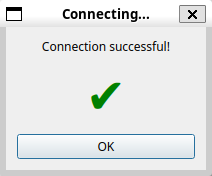
\includegraphics[width=\textwidth]{assets/figures/ConnectingSuccess.png}
        \caption{Fenêtre de connexion réussie}
        \label{fig:connecting success}
    \end{minipage}
\end{figure}

\begin{figure}[H]
    \begin{minipage}{0.64\textwidth}
        Si l'utilisateur appuie sur le bouton de connexion une fois la connexion établie, figure~\ref{fig:disconnect window}, le logiciel affiche une fenêtre de déconnexion.
        Depuis cette fenêtre, l'utilisateur peut choisir de se déconnecter du capteur QCM ou de la sonde de température, ou bien rétablir la connexion.
    \end{minipage}\hfill
    \begin{minipage}{0.30\textwidth}
        \centering
        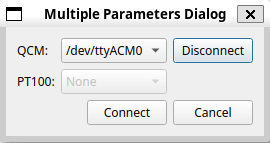
\includegraphics[width=\textwidth]{assets/figures/Disconnect.png}
        \caption{Fenêtre de déconnexion}
        \label{fig:disconnect window}
    \end{minipage}
\end{figure}

\section{Multithreading}

Le multithreading est utilisé dans le logiciel afin d'assurer la fluidité de l'interface graphique pendant les mesures.  
\fig[H, width=\textwidth]{Diagramme décrivant la relation entre les différents threads lors de la mesure}{Thread.drawio}

Le thread principal (main controller) est responsable de l'interface graphique et de la gestion des événements.  
Le thread de mesures, quant à lui, est chargé de la communication avec le capteur QCM et la sonde de température.  
Ce thread est lancé lorsque l'utilisateur appuie sur le bouton \textit{start}.  

Le thread de mesures écrit en continu les données dans des variables de signaux, tandis que le thread principal lit ces variables à intervalles réguliers (toutes les 10 ms) afin de mettre à jour l'interface graphique.

\section{Sauvegarde}

Il a été décidé de sauvegarder les données mesurées dans un fichier lisible par l'homme (human-readable) plutôt que dans un fichier binaire.  
Les deux solutions présentent des avantages et des inconvénients.

Les fichiers binaires sont plus compacts et plus rapides à lire et à écrire que les fichiers texte. Cependant, ils ne sont pas lisibles avec un simple éditeur de texte et sont moins portables entre différents systèmes.  
Pour ce projet, il a été décidé de privilégier la portabilité et la lisibilité des données, afin que celles-ci puissent être lues et comprises par d'autres personnes sans nécessiter de logiciel spécifique.

Le logiciel permet de sauvegarder les données mesurées dans un fichier au format XML.  
Les données sont organisées dans l'ordre suivant :
\begin{enumerate}
    \item Paramètres (Settings)
    \item Signal de calibration
    \item Harmoniques mesurées
    \item Autres paramètres (Parameters)
\end{enumerate}

\subsection{Performances}

Le graphe \ref{fig:LoadingPerformance} montre le temps de chargement des données en fonction de la durée de la mesure.  
On peut observer que le logiciel met environ 1000 fois moins de temps à charger les données qu'à réaliser la prise de mesures.  
Les performances de chargement des données sont donc satisfaisantes pour ce projet.

\begin{figure}[H]
    \centering
    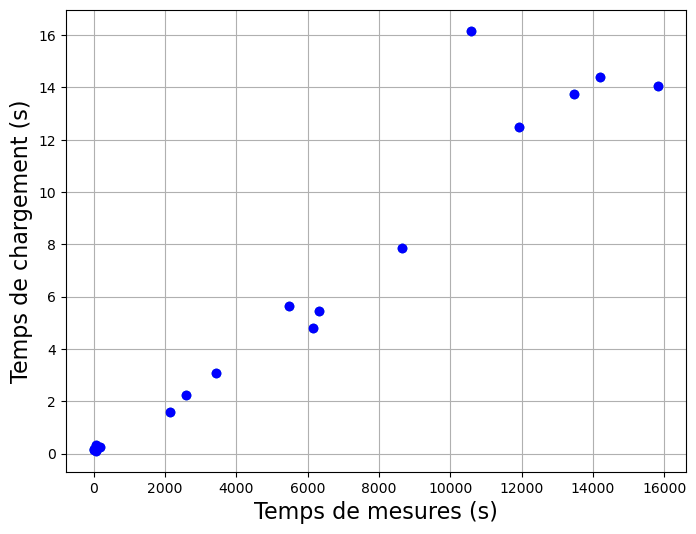
\includegraphics[width=0.8\textwidth]{assets/figures/LoadingPerformance.png}
    \caption{Temps de chargement des données}
    \label{fig:LoadingPerformance}
\end{figure}

\section{Traitement du signal}

\subsection{Filtrage du signal}

Une fois le signal mesuré, un filtre de Savitzky-Golay est appliqué pour lisser le signal et réduire le bruit.

\subsection{Interpolation des données}

Afin d'améliorer la précision des mesures, une interpolation est appliquée sur les données mesurées.

\subsection{Pics de résonance}

Les pics sont composés de la fréquence et de l'amplitude de la fréquence de résonance.  
Ces paramètres sont relativement simples à déterminer : il suffit de trouver l’échantillon du signal ayant la valeur maximale. Cette valeur correspondra à l'amplitude maximale, et l'indice de cet échantillon permet de retrouver la fréquence associée.

Un autre paramètre calculé à partir du signal est la dissipation.  
Plusieurs méthodes existent pour calculer la dissipation ; la première consiste à la déduire à partir de la constante de temps $\tau$.  
Pour cela, le quartz est soumis à une impulsion, puis une fois l'impulsion terminée, la tension aux bornes du quartz évolue sous la forme d'une oscillation amortie, comme illustré sur la figure \ref{fig:DissipationTAU}.

\subsection{Dissipation}

L'équation permettant de calculer la dissipation à partir de la constante de temps \cite{Edvardsson2024Dissipation} est la suivante :
\begin{equation}
    D = \frac{1}{2\pi f_0 \tau}
    \label{eq:Dissipation}
\end{equation}

\begin{figure}[H]
    \centering
    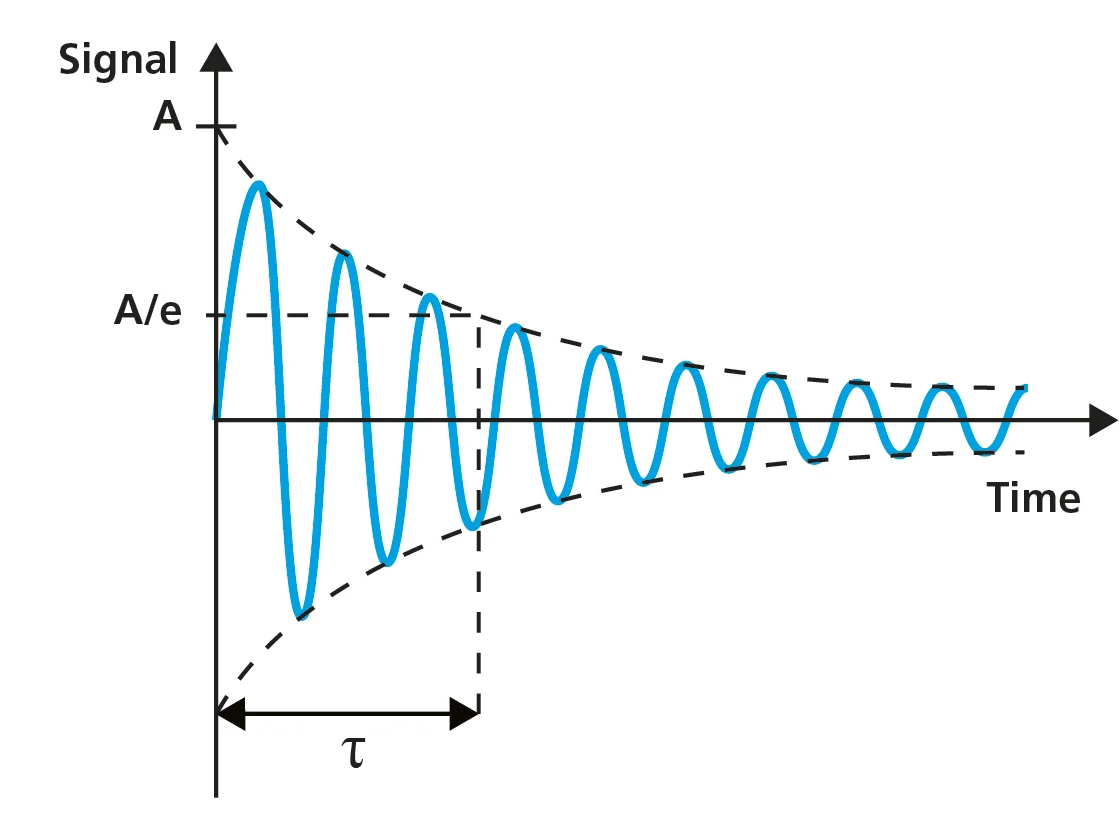
\includegraphics[width=0.8\textwidth]{assets/figures/Dissipation TAU.png}
    \caption{Oscillation amortie du quartz pour le calcul de la dissipation \cite{Edvardsson2024Dissipation}}
    \label{fig:DissipationTAU}
\end{figure}

Toutefois, cette méthode nécessite de pouvoir soumettre le quartz à une impulsion et de mesurer la constante de temps $\tau$, ce que notre capteur ne permet pas.

Une autre méthode consiste à calculer la dissipation à partir de la largeur de bande du pic de résonance.  
La largeur de bande correspond à la différence entre les fréquences aux points à -3 dB de l'amplitude maximale du pic de résonance.  
La dissipation est alors calculée à partir de la largeur de bande et de la fréquence de résonance selon l'équation suivante :
\begin{equation}
    D = \frac{BW}{f_0}
    \label{eq:DissipationWidth}
\end{equation}

\begin{figure}[H]
    \centering
    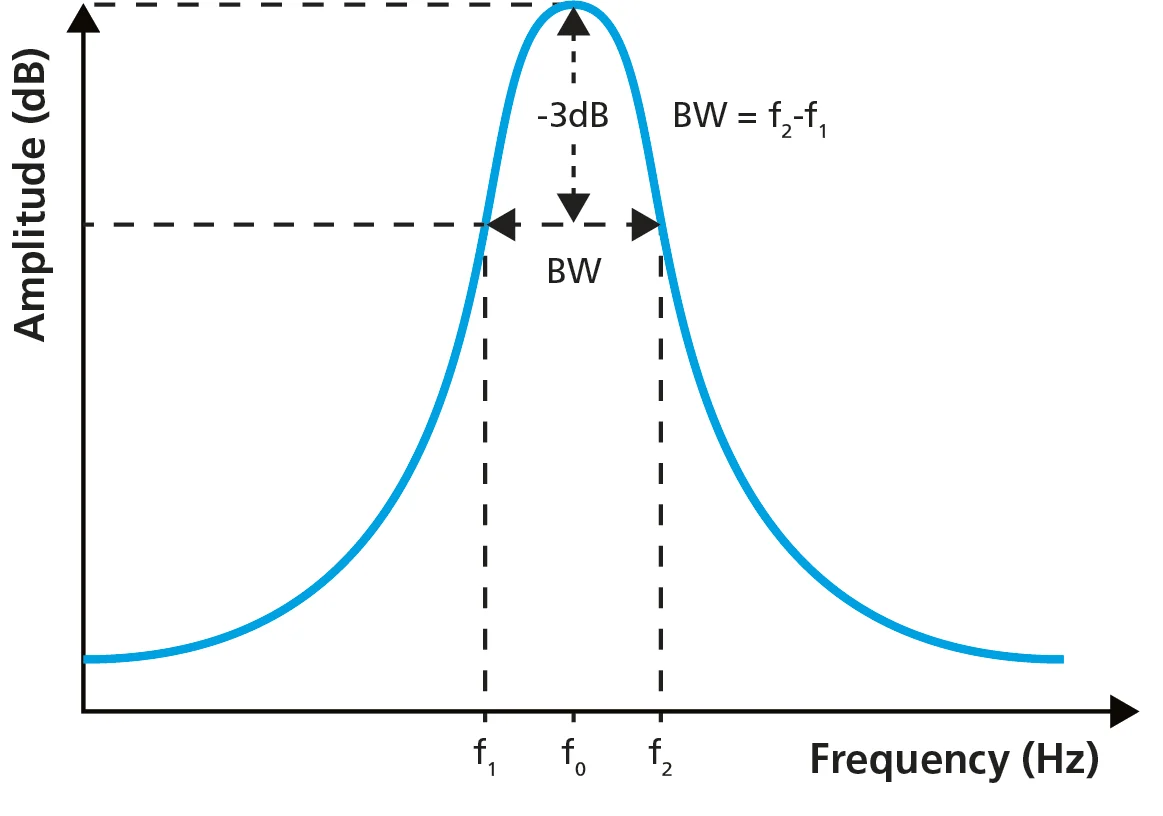
\includegraphics[width=0.8\textwidth]{assets/figures/Dissipation Capteur AMP FREQU.png}
    \caption{Amplitude du quartz pour le calcul de la dissipation \cite{Edvardsson2024Dissipation}}
    \label{fig:DissipationWidth}
\end{figure}
\newpage

